\documentclass[pdftex,11pt,a4paper]{article}
\usepackage[pdftex]{graphicx}
\usepackage{fancyhdr}
\usepackage{geometry}
\usepackage{draftcopy}
\usepackage{float}
\usepackage{amsmath}
\usepackage{algorithm2e}
\usepackage{color, colortbl}
\definecolor{Gray}{gray}{0.9}
\renewcommand{\thesection}{\arabic{section}.}
\renewcommand{\thesubsection}{\arabic{section}.\arabic{subsection} }
\renewcommand{\headrulewidth}{0pt}
\renewcommand{\footrulewidth}{0.5pt}
\pagestyle{fancy}
\fancyhead{}
\fancyfoot[LE,LO]{\footnotesize{
SE344, Chemistry and Our Environment
}
}

\title{\vspace{-15pt}Green Chemistry\\ SE344: Chemistry and Our Environment}
\author{Ankesh Kumar Singh (Y9090)}
\date{25th February, 2013}
\begin{document}
\maketitle
\begin{tabular}{p{370pt}}
\textbf{Keywords: }atom economy, synthesis of ibuprofen, Boot's process, 
\end{tabular}
\vspace{10pt}\\
\hrule
\vspace{10pt}
Ibuprofen is a commonly used analgesic and anti-inflammatory agent. It is the active ingredient in medicines tradenamed Motrin, Nuprin and Advil. It is a carboxylic acid, and its chemical name is 2-(4-isobutylphenyl)propanoic acid. Ibuprofen has a single stereomer and therefore can exist in two enantiomeric forms. The commercial product is usually the racemate. However, only the S-enantiomer is biologically active and has the desired medicinal effects. The R-enantiomer is harmless, which is fortunate, since the two enantiomers are difficult to separate. The S-enantiomer alone begins to take effect in only 12 minutes, whereas the racemate takes 38 minutes. Interestingly and luckily, the body chemically converts the inactive R-enantiomer into the active S-enantiomer.\\

A number of commercial and laboratory synthesis for racemic ibuprofen have been published. Research continues to try to improve the efficiency of each industrial process, resulting in more advantageous economics and fewer by-products (which must be disposed safely). In addition, new processes have been developed using proprietary metal catalysts to accomplish transformations not readily accomplished in the laboratory. Of particular interest are processes that will permit production and marketing of only S-enantiomer.\\

Shown here is one of the older commercial processes, developed by Boot Pure Drug Company, and a newer process, developed by the Hoechst Company. Both synthesis start with iso-butylbenzene and use Friedel Crafts acylation, but the Boot process requires six steps, while the Hoechst requires only three.\\
\begin{figure}[htb]
\centering
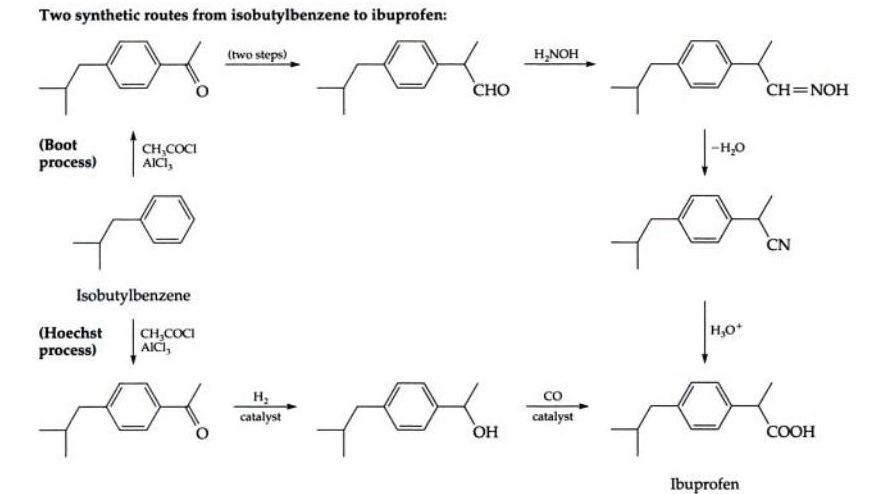
\includegraphics[clip=true,trim=0pt 0pt 0pt 0pt,scale=0.63]{ibuprofrn.png}
\end{figure} 

The ibuprofen patent ran out in the mid-1980s. Prior to that, only Boots had the right
to make and sell the drug. The patent system protects the interests of companies that
develop drugs, and allows them to sell patented drugs exclusively, normally for 20
years (although by the time the drug gets to the market, there is usually only about
ten years left to run). This allows them to recoup the money spent on a drug’s
development and also make a profit, some of which will go on investment in new
drugs.\\

\hspace{-25pt}\begin{tabular}{|p{235pt}|p{175pt}|}
\hline
Boot's process & Hoechst process\\
\hline
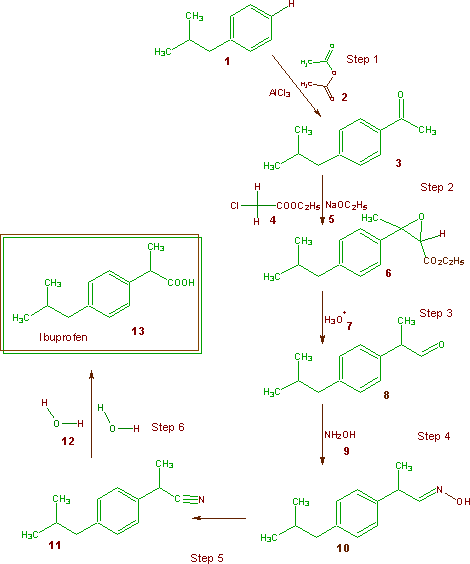
\includegraphics[clip=true,trim=0pt 0pt 0pt 0pt,scale=0.5]{ib2.png}&
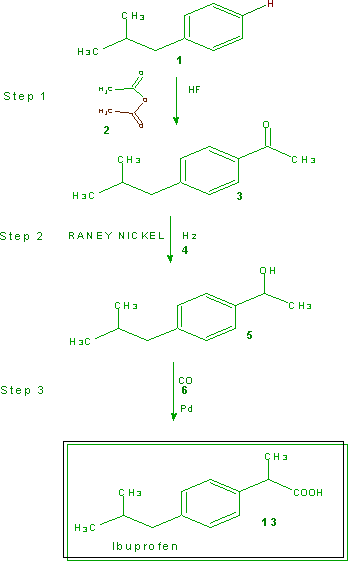
\includegraphics[clip=true,trim=0pt 0pt 0pt 0pt,scale=0.5]{ib1.png}\\
\hline
\end{tabular}
\\

Of even more importance to the green chemist than yield is atom economy, the
percentage of the raw materials and reagents used in the synthesis that actually end
up in the final product. In Boot's process, the overall figure is 40\%. This means that more than half the materials used in the
synthesis are wasted. For Hoechst process, it is 77\%, nearly double of that for Boot's process.\\

\hspace{-15pt}\begin{tabular}{p{405pt}}
\rowcolor{Gray} \vspace{-5pt} Green chemistry, also called sustainable chemistry, is a philosophy of chemical research and engineering that encourages the design of products and processes that minimize the use and generation of hazardous substances. Whereas environmental chemistry is the chemistry of the natural environment, and of pollutant chemicals in nature, green chemistry seeks to reduce and prevent pollution at its source.

As a chemical philosophy, green chemistry applies to organic chemistry, inorganic chemistry, biochemistry, analytical chemistry, and even physical chemistry. While green chemistry seems to focus on industrial applications, it does apply to any chemistry choice. 
\vspace{5pt}
\end{tabular}
\end{document}